% Provenance (never printed): 6e geography and cycle 3 sciences (locating a
% place on the globe: parallels, meridians, latitude, longitude; the Earth's
% rotation and time zones); see sources/book1/PROVENANCE.md.
% Book 1, grade 6, chapter 2.
\chapter{Latitude, longitude e fusos horários}\label{ch:g6:latitude-longitude}

A noite caiu sobre o \omterm{def:g2:water-on-earth:ocean}{oceano}. No convés de um veleiro, no ano de 1750, o
navegador levanta o seu instrumento na direção de uma estrela brilhante e
mede a que altura ela está acima do \omterm{def:g2:water-on-earth:ocean}{mar}. Alguns minutos de trabalho, e ele
sabe a que distância ao norte do \omterm{def:g3:continents-and-oceans:equator}{equador} o navio está. Mas a que
distância a leste ou a oeste? Isso ele não consegue dizer. O problema era
tão sério que, em 1714, o Parlamento britânico tinha prometido um grande
prêmio a quem encontrasse um jeito de medir isso no \omterm{def:g2:water-on-earth:ocean}{mar}. Hoje, o celular
no seu bolso dá as duas respostas em um segundo.
% ledger: rmg:15deg-per-hour, rmg:longitude-act-1714

\begin{omfigure}
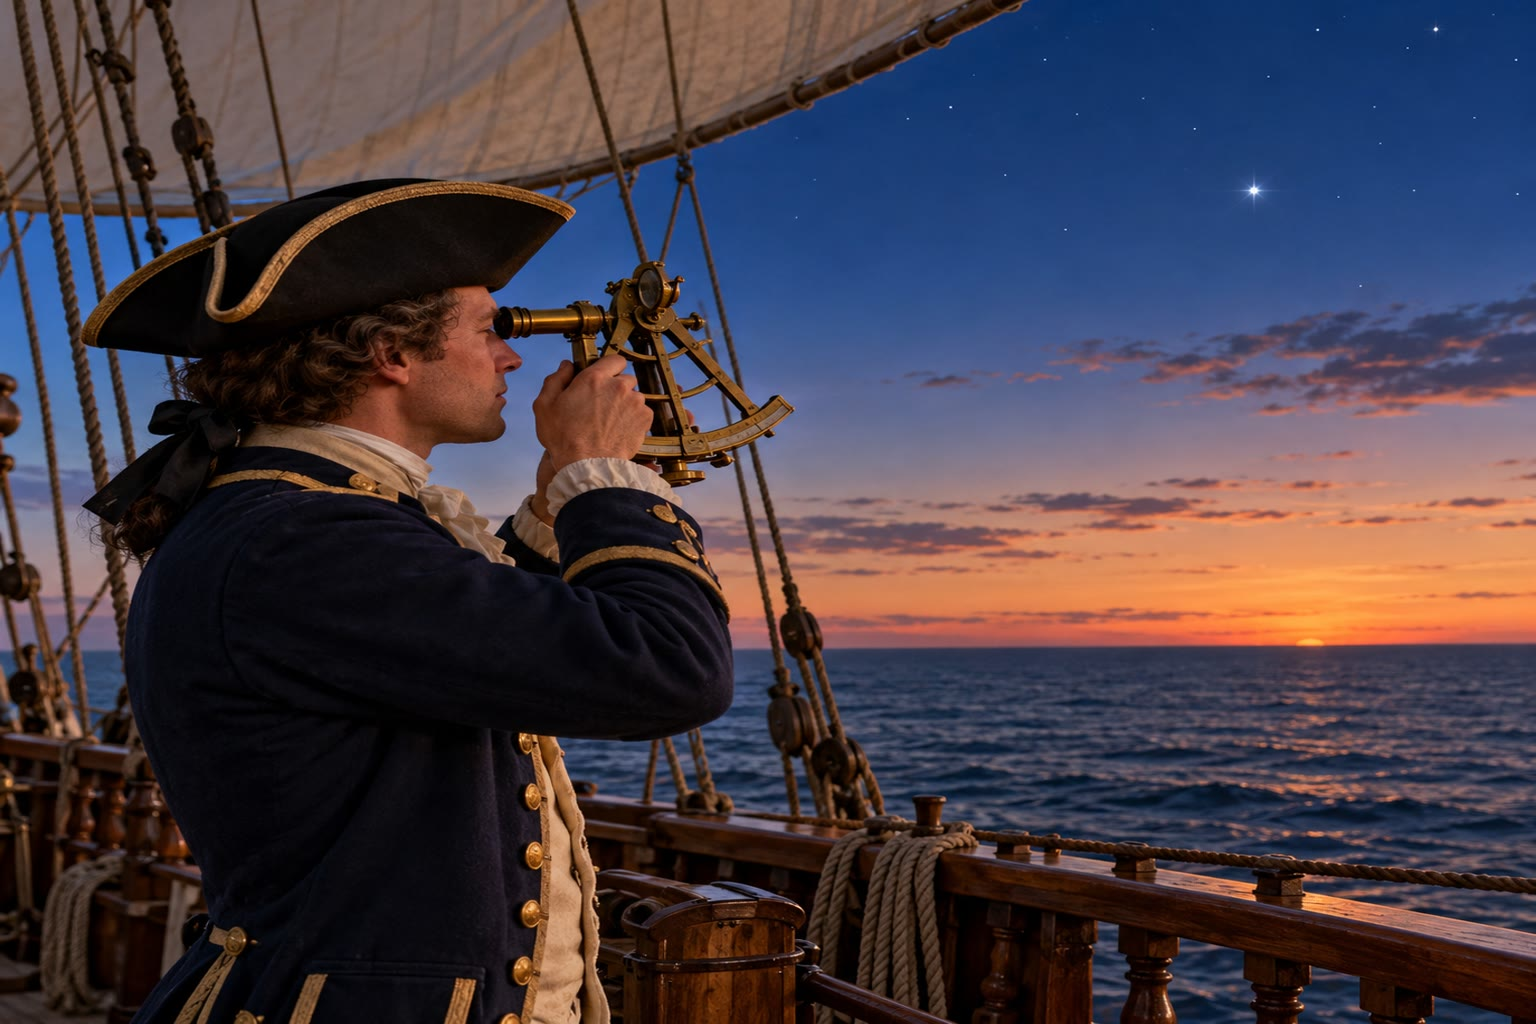
\includegraphics[width=0.62\linewidth]{images/book1/ai/g6-navigator-sextant.jpg}

{\small Um navegador do século XVIII mede a altura de uma estrela acima do
horizonte do \omterm{def:g2:water-on-earth:ocean}{mar}. (Ilustração feita por IA.)}
\end{omfigure}

\begin{recall}
Um \omterm{def:g3:continents-and-oceans:globe}{globo} é um pequeno modelo da Terra. O \omterm{def:g3:continents-and-oceans:equator}{equador} é a linha que dá a volta
no meio do \omterm{def:g3:continents-and-oceans:globe}{globo}, a meio caminho entre o \omterm{def:g3:continents-and-oceans:poles}{Polo Norte} e o \omterm{def:g3:continents-and-oceans:poles}{Polo Sul}; ele
corta a Terra em \omterm{def:g3:continents-and-oceans:equator}{hemisfério norte} e \omterm{def:g3:continents-and-oceans:equator}{hemisfério sul}
(\cref{ch:g3:continents-and-oceans}). Os livros de física mostraram que a
Terra gira sobre si mesma em torno de um eixo que passa pelos dois \omterm{def:g3:continents-and-oceans:poles}{polos},
uma vez por dia: esse giro traz o dia e a noite.
\end{recall}

\section{Os paralelos e a latitude}

Para dizer onde fica um lugar na Terra, precisamos de dois números, como a
fileira e o número de uma poltrona no cinema. O primeiro diz a que
distância ao norte ou ao sul do \omterm{def:g3:continents-and-oceans:equator}{equador} o lugar fica.

Imagine a Terra cortada em duas, passando pelos dois \omterm{def:g3:continents-and-oceans:poles}{polos}, como uma maçã
cortada do cabo para baixo. Na face do corte (à esquerda, abaixo), o
\omterm{def:g3:continents-and-oceans:equator}{equador} é a linha horizontal que passa pelo centro. Um lugar~P na
superfície é visto do centro sob um certo ângulo acima ou abaixo dessa
linha: esse ângulo é a sua \omterm{def:g6:latitude-longitude:latitude}{latitude}.

\begin{omfigure}
\begin{minipage}[t]{0.48\linewidth}\centering
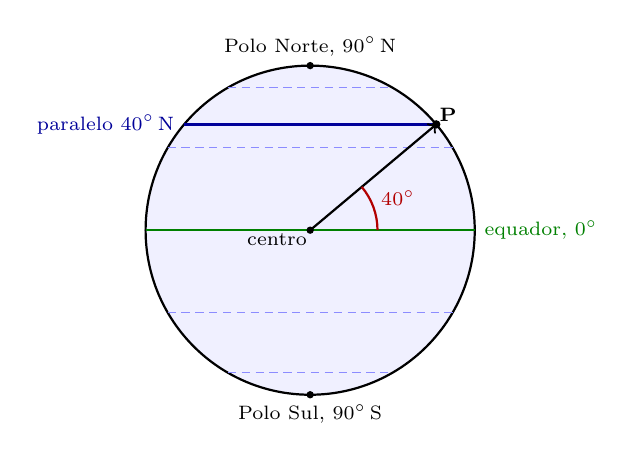
\begin{tikzpicture}[scale=0.95]
  \def\R{2.2}
  \fill[blue!6] (0,0) circle (\R);
  \draw[thick] (0,0) circle (\R);
  % parallels seen edge-on: horizontal chords
  \foreach \a in {-60,-30,30,60}{
    \draw[blue!45, densely dashed] ({-\R*cos(\a)},{\R*sin(\a)}) -- ({\R*cos(\a)},{\R*sin(\a)});}
    \draw[green!50!black, thick] (-\R,0) -- (\R,0);
  \node[font=\scriptsize, green!50!black, anchor=west] at (\R,0) {equador, $0^\circ$};
  \draw[blue!60!black, thick] ({-\R*cos(40)},{\R*sin(40)}) -- ({\R*cos(40)},{\R*sin(40)});
  \draw[->, thick] (0,0) -- ({\R*cos(40)},{\R*sin(40)});
  \fill (0,0) circle (1.4pt) node[below left, font=\scriptsize, inner sep=1pt] {centro};
  \fill ({\R*cos(40)},{\R*sin(40)}) circle (1.6pt)
    node[above right, font=\scriptsize\bfseries, inner sep=1pt] {P};
  \draw[red!70!black, thick] (0.9,0) arc (0:40:0.9);
  \node[red!70!black, font=\scriptsize] at (20:1.25) {$40^\circ$};
  \node[font=\scriptsize, blue!60!black, anchor=east] at ({-\R*cos(40)},{\R*sin(40)}) {paralelo $40^\circ$\,N};
  \fill (0,\R) circle (1.4pt) node[above, font=\scriptsize] {Polo Norte, $90^\circ$\,N};
  \fill (0,-\R) circle (1.4pt) node[below, font=\scriptsize] {Polo Sul, $90^\circ$\,S};
\end{tikzpicture}

{\small A \omterm{def:g6:latitude-longitude:latitude}{latitude}: o ângulo, no centro da Terra, entre o \omterm{def:g3:continents-and-oceans:equator}{equador} e o
lugar.}
\end{minipage}\hfill
\begin{minipage}[t]{0.48\linewidth}\centering
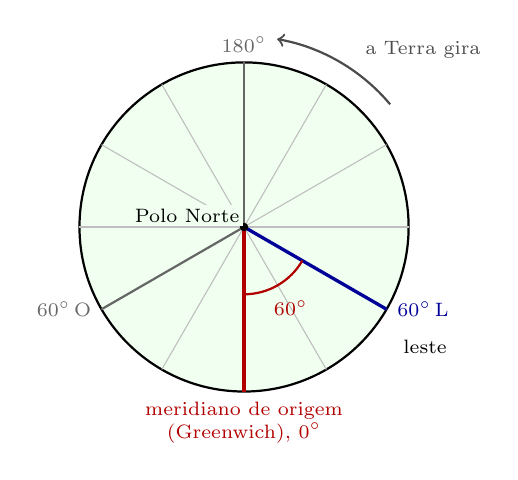
\begin{tikzpicture}[scale=0.95]
  \def\R{2.2}
  \fill[green!6] (0,0) circle (\R);
  \draw[thick] (0,0) circle (\R);
  \foreach \a in {0,30,...,330}{\draw[black!25] (0,0) -- (\a:\R);}
    \draw[red!70!black, very thick] (0,0) -- (270:\R)
    node[below, font=\scriptsize, align=center] {meridiano de origem\\(Greenwich), $0^\circ$};
  \draw[blue!60!black, very thick] (0,0) -- (330:\R)
    node[right, font=\scriptsize] {$60^\circ$\,L};
  \draw[black!60, thick] (0,0) -- (210:\R) node[left, font=\scriptsize] {$60^\circ$\,O};
  \draw[black!60, thick] (0,0) -- (90:\R) node[above, font=\scriptsize] {$180^\circ$};
  \draw[red!70!black, thick] (270:0.9) arc (270:330:0.9);
  \node[red!70!black, font=\scriptsize] at (300:1.25) {$60^\circ$};
    \fill (0,0) circle (1.6pt) node[above left, font=\scriptsize, inner sep=1.5pt, fill=green!6] {Polo Norte};
  \draw[->, thick, black!70] (40:2.55) arc (40:80:2.55);
  \node[font=\scriptsize, black!70, anchor=south west] at (55:2.6) {a Terra gira};
  \node[font=\scriptsize, anchor=west] at (2.0,-1.6) {leste $\circlearrowleft$};
\end{tikzpicture}

{\small A \omterm{def:g6:latitude-longitude:longitude}{longitude}: a Terra vista de cima do \omterm{def:g3:continents-and-oceans:poles}{Polo Norte}. O ângulo é medido
a partir do \omterm{def:g6:latitude-longitude:longitude}{meridiano de origem}, para leste ou para oeste.}
\end{minipage}
% ledger: rmg:latitude-def, rmg:longitude-def
\end{omfigure}

\begin{definition}[Paralelo e latitude]\label{def:g6:latitude-longitude:latitude}
Um \emph{paralelo}\index{paralelo} é um círculo traçado em volta do \omterm{def:g3:continents-and-oceans:globe}{globo},
paralelo ao \omterm{def:g3:continents-and-oceans:equator}{equador}; todos os lugares de um mesmo paralelo ficam à mesma
distância do \omterm{def:g3:continents-and-oceans:equator}{equador}. A \emph{latitude}\index{latitude} de um lugar é o
ângulo, medido no centro da Terra, entre o \omterm{def:g3:continents-and-oceans:equator}{equador} e esse lugar. Ela vai de
$0^\circ$ no \omterm{def:g3:continents-and-oceans:equator}{equador} a $90^\circ$ nos \omterm{def:g3:continents-and-oceans:poles}{polos}, e dizemos se o lugar fica ao
norte (N) ou ao sul (S) do \omterm{def:g3:continents-and-oceans:equator}{equador}.
% ledger: rmg:latitude-def
\end{definition}

O próprio \omterm{def:g3:continents-and-oceans:equator}{equador} é um \omterm{def:g6:latitude-longitude:latitude}{paralelo}, o mais longo, de \omterm{def:g6:latitude-longitude:latitude}{latitude} $0^\circ$. Os
\omterm{def:g6:latitude-longitude:latitude}{paralelos} ficam mais curtos na direção dos \omterm{def:g3:continents-and-oceans:poles}{polos}, e cada \omterm{def:g3:continents-and-oceans:poles}{polo} é um único
ponto, a $90^\circ$\,N ou a $90^\circ$\,S. Ao longo de uma linha que vai de
um \omterm{def:g3:continents-and-oceans:poles}{polo} ao \omterm{def:g3:continents-and-oceans:equator}{equador}, cada grau de \omterm{def:g6:latitude-longitude:latitude}{latitude} mede cerca de \qty{111}{km}.
% ledger: rmg:latitude-def

A \omterm{def:g6:latitude-longitude:latitude}{latitude} é o número fácil: ela pode ser encontrada pelo céu. De dia, os
marinheiros mediam a altura do Sol ao meio-dia; à noite, no \omterm{def:g3:continents-and-oceans:equator}{hemisfério
norte}, eles mediam a altura da Estrela Polar. É isso que o navegador da
imagem do começo está fazendo.
% ledger: rmg:15deg-per-hour

A Estrela Polar fica quase exatamente na linha do eixo da Terra,
prolongado além do \omterm{def:g3:continents-and-oceans:poles}{Polo Norte}, e tão longe que a sua luz chega a todos os
lugares da Terra ao longo de linhas paralelas. No \omterm{def:g3:continents-and-oceans:poles}{Polo Norte}, ela fica
bem a pino, a $90^\circ$ acima do horizonte; no \omterm{def:g3:continents-and-oceans:equator}{equador}, ela fica no
horizonte norte, a $0^\circ$. No meio, a regra é simples: \emph{a altura da
Estrela Polar acima do horizonte norte, medida como um ângulo, é igual à
\omterm{def:g6:latitude-longitude:latitude}{latitude}}. A figura abaixo mostra por que os dois ângulos são iguais.
% ledger: nsta:polaris-latitude

\begin{omfigure}
\begin{tikzpicture}[scale=1.1, font=\scriptsize]
  \def\R{1.7}
  \coordinate (O) at (0,0);
  \coordinate (P) at ({\R*cos(40)},{\R*sin(40)});
  \fill[blue!8] (O) circle (\R);
  \draw[black!70] (O) circle (\R);
  % equator and axis
  \draw[black!50] (-\R,0) -- (\R,0);
  \node[black!60, anchor=north east] at (-0.15,0) {equador};
  \draw[black!70, -{Stealth[length=2mm]}] (0,-\R-0.3) -- (0,\R+1.7);
  \node[anchor=east, align=right] at (-0.1,\R+1.45) {na direção da Estrela Polar\\(muito longe)};
  \node[anchor=south east] at (0,\R) {N};
  % radius to P and latitude angle at the centre
  \draw[black!80] (O) -- (P);
  \draw[red!70!black, thick] (0.55,0) arc (0:40:0.55);
  \node[red!70!black] at (20:0.8) {$40^\circ$};
  % horizon at P (tangent) and the ray to the Pole Star (parallel to the axis)
  \draw[black!70, thick] ($(P)+({-sin(40)*1.5},{cos(40)*1.5})$) -- ($(P)+({sin(40)*1.6},{-cos(40)*1.6})$);
  \node[anchor=south, rotate=-50, inner sep=2pt] at ($(P)+({sin(40)*1.15},{-cos(40)*1.15})$) {horizonte};
  \draw[orange!80!black, thick, -{Stealth[length=2mm]}] (P) -- ++(0,1.45);
  \draw[red!70!black, thick] ($(P)+(0,0.7)$) arc (90:130:0.7);
  \node[red!70!black] at ($(P)+(110:0.98)$) {$40^\circ$};
  \fill (P) circle (1.4pt);
  \node[anchor=west] at ($(P)+(0.3,0.05)$) {observador a $40^\circ$\,N};
\end{tikzpicture}

{\small Por que a altura da Estrela Polar é igual à \omterm{def:g6:latitude-longitude:latitude}{latitude} (um esboço,
fora de escala). A luz da Estrela Polar chega paralela ao eixo da Terra
(em laranja). O horizonte do observador forma um ângulo reto com o raio
que passa pelo observador; o eixo forma um ângulo reto com o \omterm{def:g3:continents-and-oceans:equator}{equador}.
Então o ângulo entre o horizonte e a Estrela Polar é o mesmo que a
\omterm{def:g6:latitude-longitude:latitude}{latitude}, o ângulo no centro entre o \omterm{def:g3:continents-and-oceans:equator}{equador} e o observador.}
% ledger: nsta:polaris-latitude
\end{omfigure}

\begin{example}[Uma navegadora à noite]\label{ex:g6:latitude-longitude:pole-star}
Uma navegadora mede a Estrela Polar a $41^\circ$ acima do horizonte norte.
O navio está na \omterm{def:g6:latitude-longitude:latitude}{latitude} $41^\circ$\,N, cerca de $41 \times 111
\approx \num{4550}$~km ao norte do \omterm{def:g3:continents-and-oceans:equator}{equador}. Navegando para o norte, ela vê
a estrela um pouco mais alta a cada noite; navegando para o sul, na
direção do \omterm{def:g3:continents-and-oceans:equator}{equador}, a estrela desce na direção do horizonte. Ao sul do
\omterm{def:g3:continents-and-oceans:equator}{equador}, a Estrela Polar não pode ser vista, porque fica abaixo do
horizonte: ali, é o Sol do meio-dia que dá a \omterm{def:g6:latitude-longitude:latitude}{latitude}.
\end{example}
% ledger: nsta:polaris-latitude, rmg:latitude-def, rmg:15deg-per-hour

\section{Os meridianos e a longitude}

O segundo número diz a que distância a leste ou a oeste um lugar fica.
Aqui não há uma linha de partida natural como o \omterm{def:g3:continents-and-oceans:equator}{equador}: é preciso escolher
uma.

\begin{definition}[Meridiano, longitude e meridiano de origem]\label{def:g6:latitude-longitude:longitude}
Um \emph{meridiano}\index{meridiano} é um semicírculo traçado no \omterm{def:g3:continents-and-oceans:globe}{globo}, do
\omterm{def:g3:continents-and-oceans:poles}{Polo Norte} ao \omterm{def:g3:continents-and-oceans:poles}{Polo Sul}. O \emph{meridiano de origem}\index{meridiano de origem}
é o meridiano escolhido como linha de partida: o que passa pelo antigo
Observatório Real de Greenwich, em Londres. A
\emph{longitude}\index{longitude} de um lugar é o ângulo entre o meridiano
de origem e o meridiano desse lugar, visto do eixo da Terra. Ela vai de
$0^\circ$ no meridiano de origem a $180^\circ$, e dizemos se o lugar fica
a leste (L) ou a oeste (O) do meridiano de origem.
% ledger: rmg:longitude-def
\end{definition}

Todos os \omterm{def:g6:latitude-longitude:longitude}{meridianos} se encontram nos \omterm{def:g3:continents-and-oceans:poles}{polos}, e todos têm o mesmo
comprimento. Do lado oposto da Terra em relação a Greenwich, o \omterm{def:g6:latitude-longitude:longitude}{meridiano}
$180^\circ$\,L e o \omterm{def:g6:latitude-longitude:longitude}{meridiano} $180^\circ$\,O são a mesma linha.

\begin{omfigure}
\begin{minipage}[c]{0.46\linewidth}\centering
\begin{tikzpicture}
  \begin{axis}[axis equal image, hide axis, width=\linewidth,
      xmin=-1.05, xmax=1.05, ymin=-1.05, ymax=1.12, clip=false]
    \fill[omSea] (axis cs:0,0) circle (1);
    \addplot[fill=omLithAlluv, draw=black!45, line width=0.2pt] table {figdata/out/grade-6-graticule-land.dat};
    \addplot[blue!50!black, line width=0.35pt] table {figdata/out/grade-6-graticule-parallels.dat};
    \addplot[black!55, line width=0.35pt] table {figdata/out/grade-6-graticule-meridians.dat};
        \addplot[green!50!black, line width=1.1pt] table {figdata/out/grade-6-graticule-equator.dat};
    \addplot[red!70!black, line width=1.1pt] table {figdata/out/grade-6-graticule-prime.dat};
    \draw[black!70] (axis cs:0,0) circle (1);
    \fill (axis cs:0,0.9063) circle (1.3pt);
        \node[font=\scriptsize, above left, inner sep=1.5pt] at (axis cs:0,0.9063) {N};
  \end{axis}
\end{tikzpicture}
\end{minipage}\hfill
\begin{minipage}[c]{0.5\linewidth}
{\small Um \omterm{def:g3:continents-and-oceans:globe}{globo} com os seus \omterm{def:g6:latitude-longitude:latitude}{paralelos} (em azul) e \omterm{def:g6:latitude-longitude:longitude}{meridianos} (em cinza),
a cada $30^\circ$. O \omterm{def:g3:continents-and-oceans:equator}{equador} está desenhado em verde grosso, e o
\omterm{def:g6:latitude-longitude:longitude}{meridiano de origem} em vermelho; eles se cruzam no \omterm{def:g2:water-on-earth:ocean}{oceano}, ao sul de Gana,
na \omterm{def:g6:latitude-longitude:latitude}{latitude} $0^\circ$, \omterm{def:g6:latitude-longitude:longitude}{longitude} $0^\circ$. Cada \omterm{def:g6:latitude-longitude:longitude}{meridiano} vai de \omterm{def:g3:continents-and-oceans:poles}{polo} a
\omterm{def:g3:continents-and-oceans:poles}{polo}; cada \omterm{def:g6:latitude-longitude:latitude}{paralelo} é um círculo em volta do eixo. (Terras: Natural Earth.)}
% ledger: data:ne-land (figdata/grade-6/graticule.py)
\end{minipage}
\end{omfigure}

\begin{history}[A escolha do meridiano de origem]
Durante muito tempo, cada país desenhou os seus \omterm{def:g2:drawing-to-map:map}{mapas} com o seu próprio
\omterm{def:g6:latitude-longitude:longitude}{meridiano} de partida: Londres, Paris e outros lugares eram usados. Em
outubro de 1884, delegados de muitos países se reuniram em Washington para
escolher um só \omterm{def:g6:latitude-longitude:longitude}{meridiano} para o mundo inteiro. Em 13~de~outubro, eles
votaram para propor o \omterm{def:g6:latitude-longitude:longitude}{meridiano} que passa pelo observatório de Greenwich:
21 países votaram a favor, um votou contra e dois não votaram.
% ledger: rmg:longitude-def, meridian:1884-vote
\end{history}

\section{Encontrar um lugar pelos seus dois ângulos}

Com a sua \omterm{def:g6:latitude-longitude:latitude}{latitude} e a sua \omterm{def:g6:latitude-longitude:longitude}{longitude}, qualquer lugar da Terra pode ser
encontrado, num \omterm{def:g2:drawing-to-map:map}{mapa} ou num \omterm{def:g3:continents-and-oceans:globe}{globo}. Escrevemos primeiro a \omterm{def:g6:latitude-longitude:latitude}{latitude}: o Cairo,
por exemplo, fica a cerca de $30^\circ$\,N, $31^\circ$\,L.
% ledger: data:b1-ne-places (figdata/grade-6/cities.py)

\begin{omfigure}
\begin{tikzpicture}
  \begin{axis}[ommap, width=\linewidth,
      xtick={-180,-150,...,180}, ytick={-90,-60,...,90},
      xticklabels={$180^\circ$,$150^\circ$O,$120^\circ$O,$90^\circ$O,$60^\circ$O,$30^\circ$O,$0^\circ$,
                   $30^\circ$L,$60^\circ$L,$90^\circ$L,$120^\circ$L,$150^\circ$L,$180^\circ$},
      yticklabels={$90^\circ$S,$60^\circ$S,$30^\circ$S,$0^\circ$,$30^\circ$N,$60^\circ$N,$90^\circ$N},
      tick label style={font=\tiny}, grid style={black!35, line width=0.3pt}]
    \addplot[fill=omLithAlluv, draw=black!45, line width=0.2pt] table {figdata/out/shared-geo-land.dat};
        \draw[green!50!black, line width=0.9pt] (axis cs:-180,0) -- (axis cs:180,0);
    \draw[red!70!black, line width=0.9pt] (axis cs:0,-90) -- (axis cs:0,90);
    \addplot[only marks, mark=*, mark size=1.2pt, black,
        point meta=explicit symbolic,
        visualization depends on={value \thisrow{anchor}\as\anc},
        nodes near coords, nodes near coords style={font=\tiny, inner sep=1.2pt,
          anchor=\anc, fill=white, fill opacity=0.75, text opacity=1}]
      table[x=lon, y=lat, meta=name, row sep=\\] {lon lat name anchor\\ -21.936 64.144 Reykjavík south\\ -0.119 51.502 Londres south\\ -73.996 40.722 Nova~York west\\ -118.232 34.049 Los~Angeles east\\ -78.502 -0.213 Quito east\\ -43.212 -22.907 Rio~de~Janeiro west\\ 18.433 -33.918 Cidade~do~Cabo north\\ 36.815 -1.281 Nairóbi west\\ 31.248 30.052 Cairo south\\ 72.876 19.068 Mumbai north\\ 139.75 35.687 Tóquio west\\ 151.213 -33.871 Sydney south\\ 174.763 -36.848 Auckland {north east}\\ };
  \end{axis}
\end{tikzpicture}

{\small Treze cidades num \omterm{def:g3:continents-and-oceans:world-map}{mapa-múndi} com uma grade a cada
$30^\circ$. O \omterm{def:g3:continents-and-oceans:equator}{equador} está desenhado em verde, e o \omterm{def:g6:latitude-longitude:longitude}{meridiano de origem} em
vermelho. (\omterm{def:g1:landscapes-around-us:water}{Litorais} e cidades: Natural Earth.)}
% ledger: data:ne-land, data:b1-ne-places (figdata/grade-6/cities.py, part map)
\end{omfigure}

\begin{method}[Localizar um lugar pelas suas coordenadas]\label{met:g6:latitude-longitude:locating}
\begin{enumerate}
  \item \omterm{def:g6:latitude-longitude:latitude}{Latitude}: parta do \omterm{def:g3:continents-and-oceans:equator}{equador} e vá para o norte (N) ou para o sul (S),
        contando os \omterm{def:g6:latitude-longitude:latitude}{paralelos}, até o número certo de graus.
  \item \omterm{def:g6:latitude-longitude:longitude}{Longitude}: parta do \omterm{def:g6:latitude-longitude:longitude}{meridiano de origem} e vá para o leste (L) ou
        para o oeste (O), contando os \omterm{def:g6:latitude-longitude:longitude}{meridianos}, até o número certo de
        graus.
  \item O lugar fica onde o \omterm{def:g6:latitude-longitude:latitude}{paralelo} e o \omterm{def:g6:latitude-longitude:longitude}{meridiano} se cruzam. Entre duas
        linhas da grade, estime: a meio caminho entre $30^\circ$ e
        $60^\circ$ fica $45^\circ$.
\end{enumerate}
\end{method}

\begin{example}[Ler as coordenadas de Sydney]\label{ex:g6:latitude-longitude:sydney}
No \omterm{def:g2:drawing-to-map:map}{mapa}, Sydney fica abaixo do \omterm{def:g3:continents-and-oceans:equator}{equador}: ela está no \omterm{def:g3:continents-and-oceans:equator}{hemisfério sul}, um
pouco acima do \omterm{def:g6:latitude-longitude:latitude}{paralelo} $30^\circ$\,S, mais perto de $30^\circ$ que de
$60^\circ$; a sua \omterm{def:g6:latitude-longitude:latitude}{latitude} é de cerca de $34^\circ$\,S. Ela fica à direita
do \omterm{def:g6:latitude-longitude:longitude}{meridiano de origem}, um pouco além do \omterm{def:g6:latitude-longitude:longitude}{meridiano} $150^\circ$\,L; a sua
\omterm{def:g6:latitude-longitude:longitude}{longitude} é de cerca de $151^\circ$\,L. Escrevemos: Sydney, $34^\circ$\,S,
$151^\circ$\,L.
% ledger: data:b1-ne-places (cities.py: 33.87 S, 151.21 E)
\end{example}

\section{A Terra que gira e os fusos horários}

A Terra gira sobre si mesma uma vez por dia, de oeste para leste. Enquanto
ela gira, o Sol parece atravessar o céu de leste para oeste. Quando o Sol
está no ponto mais alto do céu, é meio-dia. Mas não é meio-dia em todo
lugar no mesmo momento: quando é meio-dia em Londres, já é de tarde no
Cairo, mais a leste, e ainda é de manhã em Nova York, mais a oeste.

Quanto a Terra gira em uma hora? Uma volta inteira tem $360^\circ$, e ela
leva 24~horas:
\[
360^\circ \div 24 = 15^\circ \text{ por hora.}
\]
Então dois lugares separados por $15^\circ$ de \omterm{def:g6:latitude-longitude:longitude}{longitude} têm o seu
meio-dia com uma hora de diferença: o lugar mais a leste tem o meio-dia
primeiro. Um grau leva 4~minutos.
% ledger: planet:Earth.day, rmg:15deg-per-hour

\begin{definition}[Fuso horário]\label{def:g6:latitude-longitude:time-zone}
Um \emph{fuso horário}\index{fuso horario@fuso horário} é uma faixa da Terra, de \omterm{def:g3:continents-and-oceans:poles}{polo} a
\omterm{def:g3:continents-and-oceans:poles}{polo}, onde todos os relógios mostram a mesma hora. Idealmente, cada fuso
tem $15^\circ$ de \omterm{def:g6:latitude-longitude:longitude}{longitude} de largura, de modo que há 24 fusos, um para
cada hora; indo um fuso para o leste, os relógios mostram uma hora a mais.
\end{definition}

Nos fusos ideais, o fuso de um lugar é a sua \omterm{def:g6:latitude-longitude:longitude}{longitude} dividida por $15$,
arredondada para o número inteiro mais próximo: a leste de Greenwich,
somamos esse número de horas à hora de Greenwich; a oeste, subtraímos.
Tóquio, a $140^\circ$\,L: $140 \div 15 \approx 9.3$, então o fuso é $+9$:
quando é meio-dia em Greenwich, são 21~h em Tóquio. Os \omterm{def:g6:latitude-longitude:time-zone}{fusos horários} reais
não são faixas retas: eles seguem as fronteiras dos países e das regiões,
para que um país inteiro, ou uma região inteira, tenha a mesma hora.
% ledger: data:b1-ne-places, rmg:15deg-per-hour

\begin{omfigure}
\begin{tikzpicture}
  \begin{axis}[ommap, width=\linewidth, clip=false,
      xtick={-180,-90,0,90,180}, ytick={-60,0,60},
      xticklabels={$180^\circ$,$90^\circ$O,$0^\circ$,$90^\circ$L,$180^\circ$},
      yticklabels={$60^\circ$S,$0^\circ$,$60^\circ$N},
      tick label style={font=\tiny}, grid=none]
    \addplot[fill=black!8, draw=none] table {figdata/out/grade-6-time_zones-odd.dat};
    \addplot[fill=omLithAlluv, fill opacity=0.85, draw=black!45, line width=0.2pt] table {figdata/out/shared-geo-land.dat};
    \addplot[only marks, mark=none, point meta=explicit symbolic,
        nodes near coords, nodes near coords style={font=\tiny, anchor=south, inner sep=1pt}]
            table[x=lon, y=y, meta=label] {figdata/out/grade-6-time_zones-labels.dat};
    \draw[red!75!black, line width=1.6pt] (axis cs:180,-90) -- (axis cs:180,90);
    \draw[red!75!black, line width=1.6pt] (axis cs:-180,-90) -- (axis cs:-180,90);
        \draw[black, line width=0.8pt] (axis cs:0,-90) -- (axis cs:0,90);
    \node[font=\scriptsize, red!75!black, rotate=90, anchor=south] at (axis cs:180,0) {linha de data};
    \node[font=\scriptsize, red!75!black, rotate=90, anchor=north] at (axis cs:-180,0) {linha de data};
  \end{axis}
\end{tikzpicture}

{\small Os 24 \omterm{def:g6:latitude-longitude:time-zone}{fusos horários} ideais, cada um com $15^\circ$ de largura, com o
número de horas a somar à hora de Greenwich (a linha preta no meio). A
\omterm{def:g6:latitude-longitude:date-line}{linha de data} segue o \omterm{def:g6:latitude-longitude:longitude}{meridiano} de $180^\circ$, que este \omterm{def:g2:drawing-to-map:map}{mapa} corta em dois:
ele é ao mesmo tempo a borda esquerda e a borda direita. Enrole o \omterm{def:g2:drawing-to-map:map}{mapa} num
tubo, e as duas linhas vermelhas viram uma só. O fuso de cada lado da
\omterm{def:g6:latitude-longitude:date-line}{linha de data} tem meia largura.}
% ledger: rmg:15deg-per-hour, planet:Earth.day (figdata/grade-6/time_zones.py)
\end{omfigure}

\paragraph{A linha de data.} Viaje para o leste a partir de Greenwich,
somando uma hora por fuso: a $180^\circ$, você está 12~horas adiantado.
Viaje para o oeste, subtraindo uma hora por fuso: a $180^\circ$, você está
12~horas atrasado. Os dois viajantes se encontram no mesmo \omterm{def:g6:latitude-longitude:longitude}{meridiano}, com
os relógios mostrando a mesma hora, mas com um dia inteiro de diferença!
Um deles precisa mudar a data.

\begin{definition}[Linha internacional de data]\label{def:g6:latitude-longitude:date-line}
A \emph{linha internacional de data}\index{linha internacional de data} é a
linha, no meio do \omterm{def:g2:water-on-earth:ocean}{oceano} Pacífico, onde a data muda. Ela segue o \omterm{def:g6:latitude-longitude:longitude}{meridiano}
de $180^\circ$, com algumas curvas para não cortar um país em dois.
Atravessando-a para o oeste, passamos para o dia seguinte; atravessando-a
para o leste, voltamos para o dia anterior.
\end{definition}

\begin{history}[O relógio marítimo de Harrison]
\begin{minipage}[c]{0.7\linewidth}
Para encontrar a sua \omterm{def:g6:latitude-longitude:longitude}{longitude}, um navegador compara duas horas: a hora
local no navio, lida pelo Sol, e, no mesmo momento, a hora de um porto de
origem. Cada hora de diferença significa $15^\circ$ de \omterm{def:g6:latitude-longitude:longitude}{longitude}. A
dificuldade era levar a hora do porto de origem através do \omterm{def:g2:water-on-earth:ocean}{oceano}: nem os
melhores relógios da época eram precisos o bastante. O relojoeiro inglês
John Harrison passou décadas trabalhando no problema, em busca de um
relógio que não adiantasse nem atrasasse mais de 3~segundos por dia. O seu
quarto relógio marítimo, chamado H4, parece um grande relógio de bolso e
bate cinco vezes por segundo. Em 1761, o seu filho William o levou numa
viagem à Jamaica para testá-lo.
% ledger: rmg:15deg-per-hour, rmg:longitude-act-1714, rmg:h4-jamaica-1761
\end{minipage}\hfill
\begin{minipage}[c]{0.26\linewidth}\centering
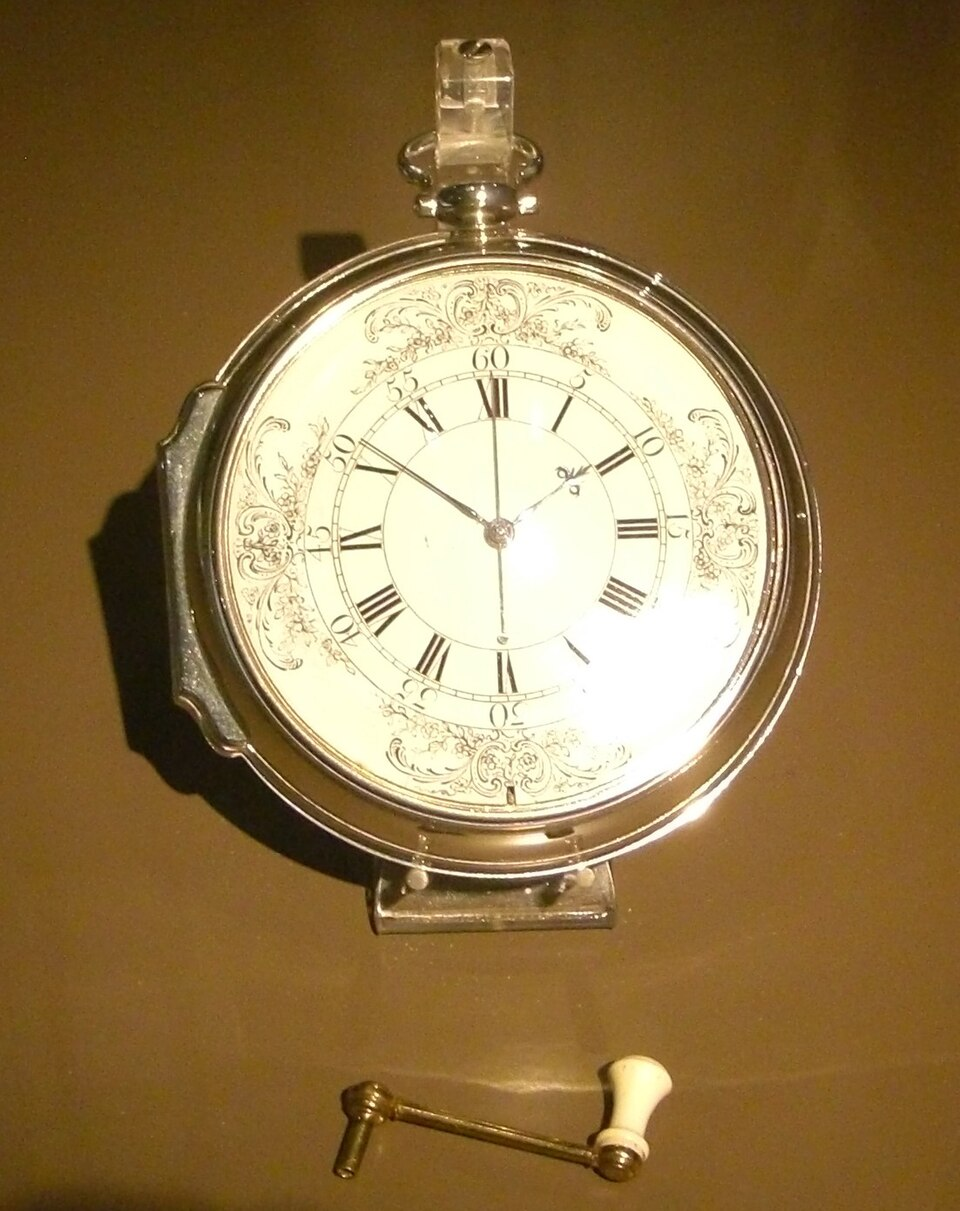
\includegraphics[width=\linewidth]{images/book1/g6-harrison-h4.jpg}\\[2pt]
{\footnotesize O H4 de Harrison, National Maritime Museum, Greenwich.
(Foto: Colonel Warden, CC BY-SA 3.0, via Wikimedia Commons.)}
% ledger: commons:harrison-h4
\end{minipage}
\end{history}

\section{Exercícios}

\begin{exercise}[$\star$]\label{exo:g6:latitude-longitude:1}
Copie e complete: ``A \omterm{def:g6:latitude-longitude:latitude}{latitude} é medida a partir do \ldots{} e vai de
$0^\circ$ a \ldots; a \omterm{def:g6:latitude-longitude:longitude}{longitude} é medida a partir do \omterm{def:g6:latitude-longitude:longitude}{meridiano} de \ldots{}
e vai de $0^\circ$ a \ldots''
\end{exercise}

\begin{exercise}[$\star$]\label{exo:g6:latitude-longitude:2}
Qual é a \omterm{def:g6:latitude-longitude:latitude}{latitude} do \omterm{def:g3:continents-and-oceans:poles}{Polo Norte}? E a do \omterm{def:g3:continents-and-oceans:poles}{Polo Sul}? E a de uma cidade no
\omterm{def:g3:continents-and-oceans:equator}{equador}?
\end{exercise}

\begin{exercise}[$\star$]\label{exo:g6:latitude-longitude:3}
Usando o \omterm{def:g2:drawing-to-map:map}{mapa} das treze cidades, diga em que \omterm{def:g3:continents-and-oceans:equator}{hemisfério}, norte ou sul, e
de que lado do \omterm{def:g6:latitude-longitude:longitude}{meridiano de origem}, leste ou oeste, fica cada uma destas
cidades: Sydney, Nova York, Cairo, Rio de Janeiro.
\end{exercise}

\begin{exercise}[$\star$]\label{exo:g6:latitude-longitude:4}
Verdadeiro ou falso? Corrija as frases falsas.
(a) Todos os \omterm{def:g6:latitude-longitude:longitude}{meridianos} se encontram nos \omterm{def:g3:continents-and-oceans:poles}{polos}.
(b) Todos os \omterm{def:g6:latitude-longitude:latitude}{paralelos} têm o mesmo comprimento.
(c) O \omterm{def:g3:continents-and-oceans:equator}{equador} é um \omterm{def:g6:latitude-longitude:latitude}{paralelo}.
(d) O \omterm{def:g6:latitude-longitude:longitude}{meridiano de origem} passa por Paris.
\end{exercise}

\begin{exercise}[$\star\star$]\label{exo:g6:latitude-longitude:5}
Usando o \omterm{def:g2:drawing-to-map:map}{mapa} das treze cidades, qual cidade fica a cerca de
$30^\circ$\,N, $31^\circ$\,L? Qual fica a cerca de $41^\circ$\,N,
$74^\circ$\,O? Dê as coordenadas aproximadas de Tóquio.
% ledger: data:b1-ne-places (cities.py main table)
\end{exercise}

\begin{exercise}[$\star\star$]\label{exo:g6:latitude-longitude:6}
A cidade~A fica na \omterm{def:g6:latitude-longitude:longitude}{longitude} $0^\circ$, e a cidade~B na \omterm{def:g6:latitude-longitude:longitude}{longitude}
$45^\circ$\,L. Quantas horas separam os seus meios-dias? Em que cidade é
meio-dia primeiro?
\end{exercise}

\begin{exercise}[$\star\star$]\label{exo:g6:latitude-longitude:7}
Mumbai fica a cerca de $73^\circ$\,L. Calcule o seu \omterm{def:g6:latitude-longitude:time-zone}{fuso horário} ideal.
Quando é meio-dia em Greenwich, que horas são em Mumbai, nos fusos ideais?
% ledger: data:b1-ne-places (cities.py: 72.88 E, zone +5)
\end{exercise}

\begin{exercise}[$\star\star$]\label{exo:g6:latitude-longitude:8}
Cada grau de \omterm{def:g6:latitude-longitude:latitude}{latitude} mede cerca de \qty{111}{km}. A que distância do
\omterm{def:g3:continents-and-oceans:equator}{equador} fica uma cidade a $30^\circ$\,N, medindo ao longo do seu \omterm{def:g6:latitude-longitude:longitude}{meridiano}?
A que distância o \omterm{def:g3:continents-and-oceans:poles}{Polo Norte} fica do \omterm{def:g3:continents-and-oceans:equator}{equador}?
% ledger: rmg:latitude-def
\end{exercise}

\begin{exercise}[$\star\star$]\label{exo:g6:latitude-longitude:9}
Nova York fica no fuso $-5$, e Tóquio no fuso $+9$. Quantas horas separam
os seus relógios? Quando são 8~h de segunda-feira em Nova York, que horas
são, e que dia é, em Tóquio?
% ledger: data:b1-ne-places (cities.py: zones -5 and +9)
\end{exercise}

\begin{exercise}[$\star\star$]\label{exo:g6:latitude-longitude:10}
Lena diz: ``O Sol nasce no leste, então as cidades do leste veem o Sol
nascer antes das cidades do oeste.'' Ela tem razão? Explique com o giro da
Terra.
\end{exercise}

\begin{exercise}[$\star\star\star$]\label{exo:g6:latitude-longitude:11}
O relógio de um navio adianta 3~segundos por dia (ele anda rápido demais).
(a) Quantos segundos adiantado ele está depois de uma viagem de 42~dias?
(b) A Terra gira um grau em 4~minutos, ou seja, 240~segundos. Que erro, em
graus de \omterm{def:g6:latitude-longitude:longitude}{longitude}, o erro do relógio provoca? (c) No \omterm{def:g3:continents-and-oceans:equator}{equador}, um grau de
\omterm{def:g6:latitude-longitude:longitude}{longitude} mede cerca de \qty{111}{km}. Em cerca de quantos quilômetros o
navegador se engana, no \omterm{def:g3:continents-and-oceans:equator}{equador}?
% ledger: rmg:longitude-act-1714, rmg:15deg-per-hour, rmg:latitude-def
\end{exercise}

\begin{exercise}[$\star\star\star$]\label{exo:g6:latitude-longitude:12}
Um avião sai de Tóquio (fuso $+9$) às 18~h de segunda-feira e voa para o
leste, atravessando o Pacífico, até Los Angeles (fuso $-8$). O voo dura
10~horas. (a) Que horas são em Greenwich quando o avião parte? (b) Que
horas são em Greenwich quando ele pousa? (c) Qual é a hora local e o dia
em Los Angeles quando ele pousa? Por que os viajantes dizem que, nesse
voo, ``você pousa antes de ter decolado''?
\end{exercise}

\section{Problema: Uma chamada de vídeo em volta do mundo}

\begin{problem}[{Problema de fim de semana --- cinco amigos, quatro fusos
horários e uma linha de data: que horas são em Auckland quando a chamada
começa?}]
\label{pb:g6:latitude-longitude:1}
% ledger: data:b1-ne-places, rmg:15deg-per-hour, planet:Earth.day (cities.py, time_zones.py; test_cities_zones_used_in_the_problem)
Lena mora em Londres. Ela quer organizar uma chamada de vídeo com quatro
amigos que conheceu nas férias: Ana, no Rio de Janeiro, Kenji, em Tóquio,
Mia, em Auckland, e Sam, em Los Angeles. Neste problema, usamos os \omterm{def:g6:latitude-longitude:time-zone}{fusos
horários} ideais.

\begin{center}
\small
\begin{tabular}{lll}
\hline
amigo & cidade & coordenadas\\
\hline
Lena & Londres & $52^\circ$\,N, $0^\circ$\\
Ana & Rio de Janeiro & $23^\circ$\,S, $43^\circ$\,O\\
Kenji & Tóquio & $36^\circ$\,N, $140^\circ$\,L\\
Mia & Auckland & $37^\circ$\,S, $175^\circ$\,L\\
Sam & Los Angeles & $34^\circ$\,N, $118^\circ$\,O\\
\hline
\end{tabular}
\end{center}

\medskip
\noindent\textbf{Parte I --- Onde os amigos moram.}
\begin{enumerate}
  \item Quais amigos moram no \omterm{def:g3:continents-and-oceans:equator}{hemisfério sul}?
  \item Quais amigos moram a oeste do \omterm{def:g6:latitude-longitude:longitude}{meridiano de origem}?
  \item Qual amigo mora mais longe do \omterm{def:g3:continents-and-oceans:equator}{equador}?
  \item Qual amigo mora mais perto do \omterm{def:g6:latitude-longitude:longitude}{meridiano} de $180^\circ$? A quantos
        graus de \omterm{def:g6:latitude-longitude:longitude}{longitude} dele?
\end{enumerate}

\medskip
\noindent\textbf{Parte II --- Que horas são?}
\begin{enumerate}[resume]
  \item Quantos graus a Terra gira em uma hora?
  \item Calcule o \omterm{def:g6:latitude-longitude:time-zone}{fuso horário} ideal da cidade de cada amigo.
  \item Lena propõe começar a chamada na sexta-feira, às 20~h, hora de
        Londres. Que horas são, e que dia é, no Rio de Janeiro? E em Tóquio?
  \item Kenji responde que vai estar dormindo. Explique por que já é
        sábado em Tóquio.
\end{enumerate}

\medskip
\noindent\textbf{Parte III --- Atravessar a linha de data.}
\begin{enumerate}[resume]
  \item Que horas são, e que dia é, em Los Angeles quando a chamada começa?
  \item Quantas horas os relógios de Auckland estão adiantados em relação
        aos de Los Angeles?
  \item Navegando para o leste, de Auckland a Los Angeles, um navio
        atravessa a \omterm{def:g6:latitude-longitude:date-line}{linha de data}. Ele avança para o dia seguinte ou volta
        para o dia anterior?
  \item Qual é a hora local, e o dia, em Auckland quando a chamada começa?
\end{enumerate}
\end{problem}
